\documentclass[12pt]{article}

% a template that a friend gave, it's worked well enough for me
% i have added some packages and stuff that have proved useful

\usepackage{fancyhdr}
\usepackage{tipa}
\usepackage{fontspec}
\usepackage{amsfonts}
\usepackage{enumitem}
\usepackage[margin=1in]{geometry}
\usepackage{graphicx}
\usepackage{float}
\usepackage{amsmath}
\usepackage{braket}
\usepackage{amssymb}
\usepackage{booktabs}
\usepackage{hyperref}
\usepackage{mathtools}
\usepackage{xcolor}
\usepackage{float}
\usepackage{algpseudocodex}
\usepackage{titlesec}
\usepackage{bbm}

\pagestyle{fancy}
\fancyhf{} % sets both header and footer to nothing
\lhead{Kevin Sheng}
\setmainfont{Comic Neue}
\renewcommand{\headrulewidth}{1pt}
\setlength{\headheight}{0.75in}
\setlength{\oddsidemargin}{0in}
\setlength{\evensidemargin}{0in}
\setlength{\voffset}{-.5in}
\setlength{\headsep}{10pt}
\setlength{\textwidth}{6.5in}
\setlength{\headwidth}{6.5in}
\setlength{\textheight}{8in}
\renewcommand{\headrulewidth}{0.5pt}
\renewcommand{\footrulewidth}{0.3pt}
\setlength{\textwidth}{6.5in}
\usepackage{setspace}
\usepackage{multicol}
\usepackage{float}
\setlength{\columnsep}{1cm}
\setlength\parindent{24pt}
\usepackage [english]{babel}
\usepackage [autostyle, english = american]{csquotes}
\MakeOuterQuote{"}

\setlength{\parskip}{6pt}
\setlength{\parindent}{0pt}

\titlespacing\section{0pt}{12pt plus 4pt minus 2pt}{0pt plus 2pt minus 2pt}
\titlespacing\subsection{0pt}{12pt plus 4pt minus 2pt}{0pt plus 2pt minus 2pt}
\titlespacing\subsubsection{0pt}{12pt plus 4pt minus 2pt}{0pt plus 2pt minus 2pt}

\hypersetup{colorlinks=true, urlcolor=blue}

\newcommand{\correction}[1]{\textcolor{red}{#1}}


\rhead{ECE 102}

\newcommand{\rect}{\operatorname{rect}}
\newcommand{\sinc}{\operatorname{sinc}}
\newcommand{\ft}[1]{\mathcal{F}\left[#1\right]}
\newcommand{\ift}[1]{\mathcal{F}^{-1}\left[#1\right]}
\newcommand{\lt}[1]{\mathcal{L}\left[#1\right]}
\newcommand{\ilt}[1]{\mathcal{L}^{-1}\left[#1\right]}


\begin{document}
\begin{enumerate}
      \item \begin{enumerate}
                  \item The bandwidth of this signal is $B=2$, so the Nyquist rate is $2B=\boxed{4\text{ Hz}}$.
                  \item $F_s=0.5\text{ Hz} \rightarrow \omega_0=\pi$: \\
                        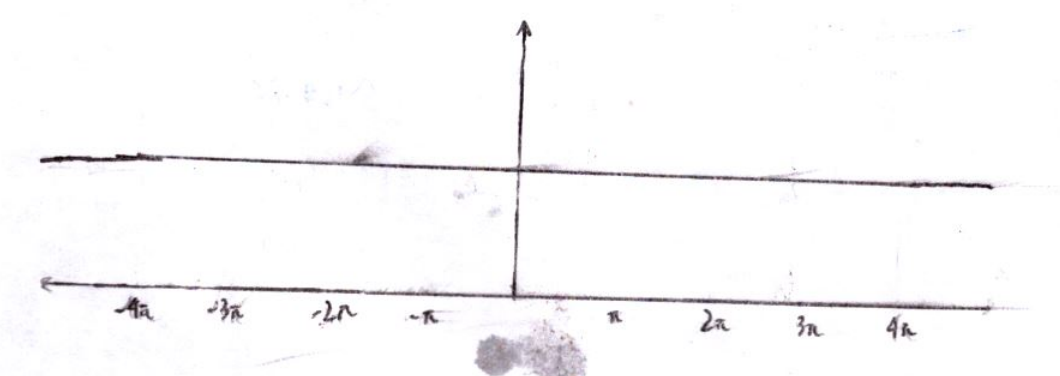
\includegraphics[width=10cm]{img/hw7/half_hertz}

                        $F_s=1\text{ Hz} \rightarrow \omega_0=2\pi$: \\
                        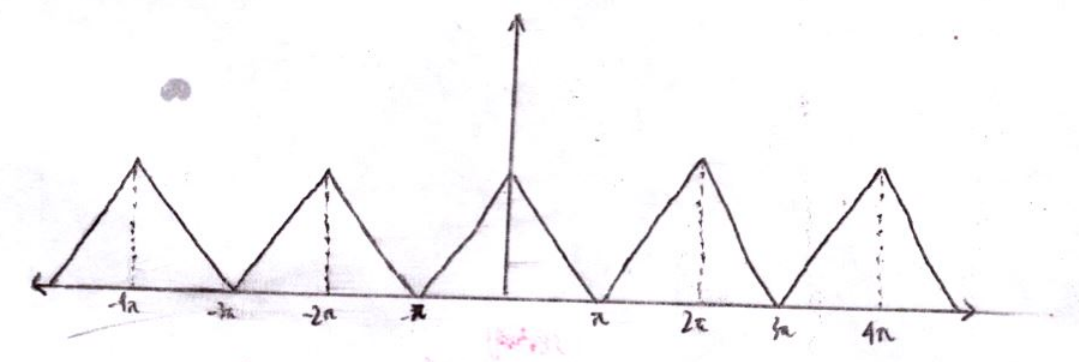
\includegraphics[width=10cm]{img/hw7/one_hertz}

                        As we can see, only the first one has aliasing.
                        To get $F_s$ out of the sampled second one, we can use a bandpass
                        filter with centers at $\pm \frac{7\pi}{2}$ and a width of $\pi$.
            \end{enumerate}
      \item \begin{enumerate}
                  \item $\tilde{f}(t)=f(t)(\delta_2(t)+\delta_2(t-(1+\tau)))$
                  \item \[\begin{aligned}
                                    \ft{\tilde{f}(t)}
                                     & = \ft{f(t)\delta_2(t)}+\ft{f(t)\delta_2(t-1-\tau)}                                                                                           \\
                                     & = \frac{1}{2} \left(F(j\omega) * \delta_{\pi}(\omega)+F(j\omega) * \left(\delta_{\pi}(\omega)e^{-j\omega(1+\tau)}\right)\right)              \\
                                     & = \frac{1}{2} \sum_{k=-\infty}^{\infty} F(j\omega) * \delta(\omega-k\pi) + F(j\omega) * \left(\delta(\omega-k\pi)e^{-j\omega(1+\tau)}\right) \\
                                     & = \frac{1}{2} \sum_{k=-\infty}^{\infty} F(j(\omega-k\pi))+F(j(\omega-k\pi))e^{-jk\pi(1+\tau)}                                                \\
                                     & = \frac{1}{2} \sum_{k=-\infty}^{\infty} F(j(\omega-k\pi))\left(1+e^{-jk\pi(1+\tau)}\right)
                              \end{aligned}\] \label{list:2b}
                              And future me is realizing that this is not what the question was asking.
                              Thankfully, we can plug in $\ft{1}=2\pi\delta(\omega)$ to find that
                              \[\boxed{\ft{f(t)}=\pi \sum_{k=-\infty}^{\infty} \delta(\omega-k\pi)\left(1+e^{-jk\pi(1+\tau)}\right)}\]
                              
                  \item When $\tau=0$, our summation becomes
                        \[\frac{1}{2} \sum_{k=-\infty}^{\infty} F(j(\omega-k\pi))\left(1+e^{-jk\pi}\right)\]
                        Notice that at even $k$, $e^{-jk\pi}=1$, while at odd $k$, $e^{-jk\pi}=-1$.

                        Because of this, we can rewrite the summation as
                        \[\frac{1}{2} \sum_{k=-\infty}^{\infty} 2F(j(\omega-2k\pi))=\sum_{k=-\infty}^{\infty} F(j(\omega-2k\pi))\]
                        which is the same thing we get as when we evaluate $\ft{f(t)\delta_1(t)}$.
                  \item 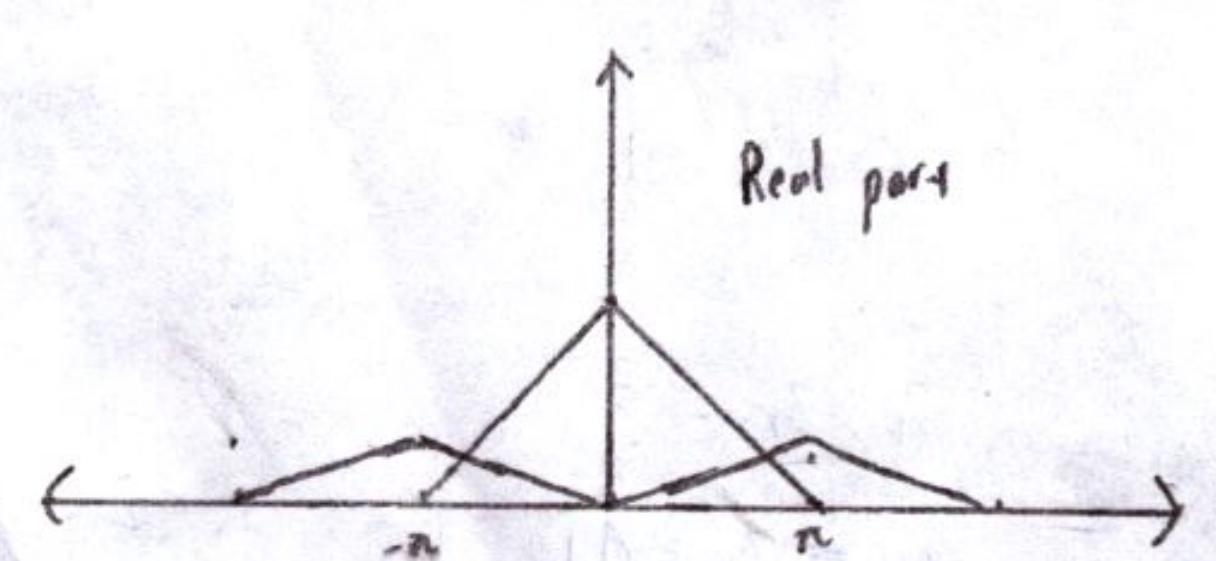
\includegraphics[width=7cm]{img/hw7/sampled_g_re}
                        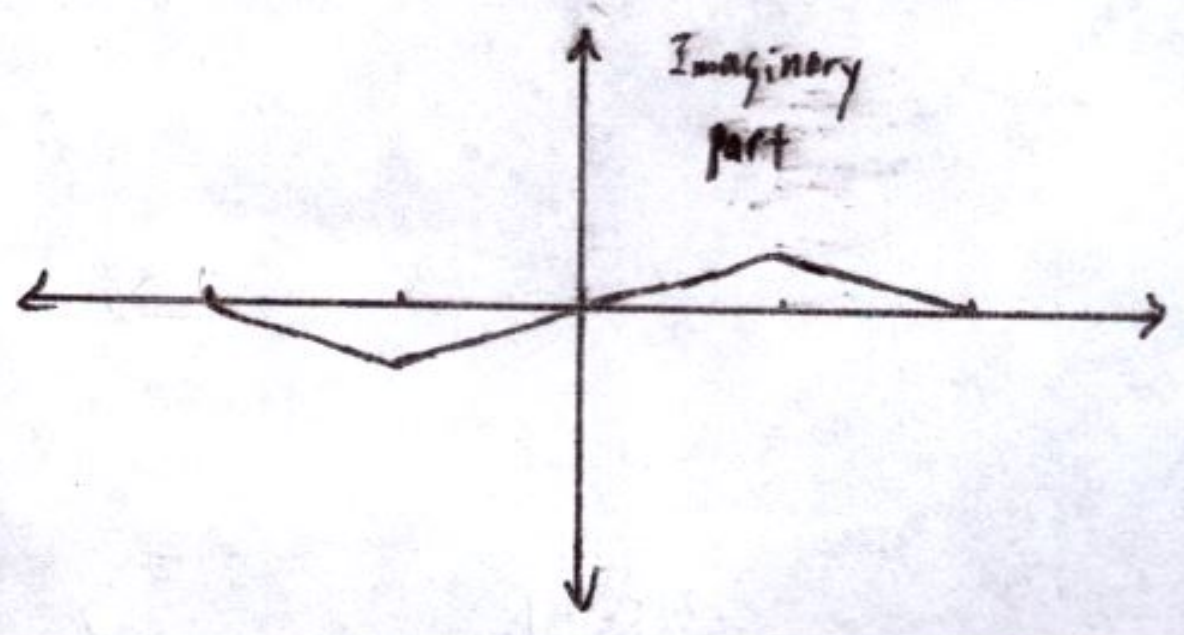
\includegraphics[width=7cm]{img/hw7/sampled_g_im}
                  \item We can recover an approximation of $g(t)$ since although
                        there is aliasing in the real part, the replicas don't interfere in the imaginary part.
            \end{enumerate}
      \item \begin{enumerate}
                  \item By a similar process to what we did in \ref{list:2b}, we have
                        \[X_p(j\omega)=\frac{1}{2\Delta}\sum_{k=-\infty}^{\infty} F\left(jw-\frac{k\pi}{\Delta}\right)\left(1-e^{-jk\pi}\right)\]
                        This only preserves odd $k$, as at even $k$ $e^{-jk\pi}=1$ and the term becomes $0$.

                        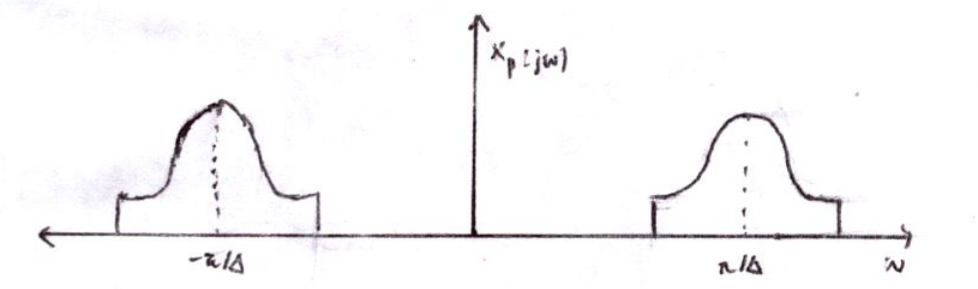
\includegraphics[width=12cm]{img/hw7/sampled_sig}
                  \item To recover $x(t)$ from $x_p(t)$, we could first put it through a modulator
                        \[\mathcal{S}[x(t)]=x(t)\cos\left(\frac{\pi}{\Delta}t\right)\]
                        then convolve with with a LPF with width $2\omega_m$ and height $\Delta$.
                  \item We can do the same thing with $y(t)$.
                        The only thing that changes is that the height of the LPF should now be $2\Delta$.
                  \item For there to not be aliasing betwen the differnet copies,
                        we need at least $2\omega_m$ of space between the periods.
                        The centers are spaced $\frac{2\pi}{\Delta}$ apart, so we have
                        \[\frac{2\pi}{\Delta} \ge 2\omega_m \rightarrow \boxed{\Delta \le \frac{\pi}{\omega_m}}\]
            \end{enumerate}
      \item \begin{enumerate}
                  \item \begin{enumerate}
                              \item \[\begin{aligned}
                                                \lt{f(t)}
                                                 & = \lt{e^{-at}t \cdot \frac{1-\cos 2\omega_0t}{2}}                       \\
                                                 & = \left(\lt{e^{-at}t}-\lt{e^{-at}t\cos 2\omega_0t}\right) \div 2         \\
                                                 & = \left(\lt{e^{-at}t}+\frac{d}{ds}\lt{e^{-at}\cos 2\omega_0t}\right) \div 2         \\
                                                 & = \left(\frac{1}{(s+a)^2}+\frac{d}{ds}\frac{s+a}{(s+a)^2+4\omega_0^2}\right) \div 2 \\
                                                 & = \left(\frac{1}{(s+a)^2}+\frac{4\omega_0^2-(s+a)^2}{\left((s+a)^2+4\omega_0^2\right)^2}\right) \div 2 \\
                                                 & = \boxed{\frac{1}{2(s+a)^2}-\frac{4\omega_0^2-(s+a)^2}{2\left((s+a)^2+4\omega_0^2\right)^2}}
                                          \end{aligned}\]
                                    The ROC of the first one is $\Re(s) > -a$.
                                    The second one turns from $\Re(s) > 0$ to the same one as the first one,
                                    so the total ROC is $\boxed{\Re(s) > -a}$.
                              \item \[\begin{aligned}
                                                \lt{f(t)}
                                                 & = \int_{0}^{\infty} e^{-b|t|}e^{-st}\,dt                       \\
                                                 & = \int_{0}^{\infty} e^{-t(b+s)}\,dt                            \\
                                                 & = \left.\left(-\frac{1}{b+s}e^{-t(b+s)}\right)\right|^\infty_0 \\
                                                 & = \boxed{\frac{1}{b+s}}
                                          \end{aligned}\]
                                    For the integral to converge, we need $\Re(b+s)>0$,
                                    so our ROC is $\boxed{\Re(s)>b}$.
                        \end{enumerate}
                  \item $\lt{x(t)e^{s_0t}}=X(s-s_0)$, given that $\Re(s-s_0)>-1$.
                        \begin{enumerate}
                              \item \[\begin{aligned}
                                                X\left(j\omega-\frac{1}{2}\right)
                                                 & = \frac{1}{\left(j\omega-\frac{1}{2}\right)^2+2\left(j\omega-\frac{1}{2}\right)+5} \\
                                                 & = \boxed{\frac{1}{-\omega^2+j\omega+\frac{17}{4}}}
                                          \end{aligned}\]
                              \item $\Re(s-s_0)=-2 < -1$, so the FT isn't in the ROC and we can't oneshot it.
                        \end{enumerate}
            \end{enumerate}
      \item \begin{enumerate}
                  \item $\lt{f(t-1)}=e^{-s}F(s)$,
                        so we can ILT the rational fraction independently.
                        \begin{gather*}
                              \frac{s+1}{(s-2)^2(s-3)} = \frac{r_1}{s-2}+\frac{r_2}{(s-2)^2}+\frac{s_3}{s-3} \\
                              s+1=r_1(s-2)(s-3)+r_2(s-3)+r_3(s-2)^2 \\
                              s+1=r_1(s-2)(s-3)+r_2(s-3)-r_1(s-2)^2 \\
                              s+1=r_1(2-s)+r_2(s-3)
                        \end{gather*}
                        Solving the linear equations given allows us to obtain
                        \[\frac{s+1}{(s-2)^2(s-3)}=-\frac{4}{s-2}-\frac{3}{(s-2)^2}+\frac{4}{s-3}\]
                        The ILT of this is
                        \[u(t)\left(-4e^{2t}-3te^{2t}-4e^{3t}\right)\]
                        Noting that this is actually $f(t-1)$, our actual ILT is
                        \[\boxed{u(t-1)\left(-4e^{2t-2}-3te^{2t-2}-4e^{3t-3}\right)}\]

                  \item We use the linear algebra method:
                        \begin{gather*}
                              \frac{s+4}{s(s+2j)(s-2j)}=\frac{r_1}{s}+\frac{r_2}{s+2j}+\frac{r_3}{s-2j} \\
                              s+4=r_1(s^2+4)+r_2(s^2-2js)+r_3(s^2+2js)
                        \end{gather*}

                        This gives us the following set of equations:
                        \begin{gather*}
                              \sum r_i=0 \\
                              4r_1=4 \\
                              -2jr_2+2jr_3=1
                        \end{gather*}
                        Solving, we find
                        \begin{align*}
                              r_1=1 &  & r_2=-\frac{1}{2}-\frac{1}{4j} &  & r_3=-\frac{1}{2}+\frac{1}{4j}
                        \end{align*}
                        and using $\ilt{\frac{1}{s-\lambda}}=u(t)e^{\lambda}$ gives us
                        \begin{align*}
                              \ilt{F(s)}
                              &=u(t)\left(1+\left(-\frac{1}{2}-\frac{1}{4j}\right)e^{-2jt}+\left(-\frac{1}{2}+\frac{1}{4j}\right)e^{2jt}\right) \\
                              &=u(t)\left(1+\left(-\frac{1}{2}+\frac{j}{4}\right)e^{-2jt}+\left(-\frac{1}{2}-\frac{j}{4}\right)e^{2jt}\right) \\
                              &=u(t)\left(1-\cos(2t)+\frac{1}{2}\sin(2t)\right)
                        \end{align*}
            \end{enumerate}
      \item \begin{enumerate}
                  \item The transfer function is
                        \[H(s)=\frac{a}{s^2+5s+4}\]
                        It remains to figure out $a$.
                        Using the given input-output pair, we know $H(s=1)=\frac{1}{2}$,
                        so $a=\frac{1}{2} \cdot 10=5$ and our actual transfer function is
                        \[\boxed{H(s)=\frac{5}{(s+1)(s+4)}}\]
                  \item $\lt{u(t)}=\frac{1}{s}$, so $Y(s)=\frac{5}{s(s+1)(s+4)}$.
                        We ILT this by doing PFD.
                        \begin{gather*}
                              \frac{5}{s(s+1)(s+4)}=\frac{r_1}{s}+\frac{r_2}{s+1}+\frac{r_3}{s+4} \\
                              \begin{aligned}
                                    r_1=\frac{5}{(0+1)(0+4)}=\frac{5}{4}  &  &
                                    r_2=\frac{5}{(-1)(-1+4)}=-\frac{5}{3} &  &
                                    r_3=\frac{5}{(-4)(-4+1)}=\frac{5}{12}
                              \end{aligned}
                        \end{gather*}
                        Applying the ILT to each of these individually gives
                        \[\boxed{y(t)=u(t)\left(\frac{5}{4}-\frac{5}{3}e^{-t}+\frac{5}{12}e^{-4t}\right)}\]
                  \item The LT of the input is
                        \[\frac{1}{s}-\frac{e^{-s}}{s}\]
                        and since $r(t)=u(t)t$, the LT of the output is
                        \[\frac{1}{s^2}-\frac{2e^{-s}}{s^2}+\frac{e^{-2s}}{s^2}
                              =\frac{\left(e^{-s}-1\right)^2}{s^2}\]
                        from these two we get that the transfer function of $\mathcal{S}_2$ is
                        \[H_2(s)=\frac{1-e^{-s}}{s}\]
                        and the transfer function of the two systems combined is
                        \[H(s)=\frac{5-5e^{-s}}{s(s+1)(s+4)}\]
                        Using the same PFD as in the previous part, we get our impulse response
                        \[\boxed{h(t)=u(t)\left(\frac{5}{4}-\frac{5}{3}e^{-t}+\frac{5}{12}e^{-4t}\right)
                        -u(t-1)\left(\frac{5}{4}-\frac{5}{3}e^{-t+1}+\frac{5}{12}e^{-4t+4}\right)}\]
            \end{enumerate}
\end{enumerate}
\end{document}
